%
% Complete documentation on the extended LaTeX markup used for Insight
% documentation is available in ``Documenting Insight'', which is part
% of the standard documentation for Insight.  It may be found online
% at:
%
%     http://www.itk.org/

\documentclass{InsightArticle}

\usepackage[dvips]{graphicx}

%%%%%%%%%%%%%%%%%%%%%%%%%%%%%%%%%%%%%%%%%%%%%%%%%%%%%%%%%%%%%%%%%%
%
%  hyperref should be the last package to be loaded.
%
%%%%%%%%%%%%%%%%%%%%%%%%%%%%%%%%%%%%%%%%%%%%%%%%%%%%%%%%%%%%%%%%%%
\usepackage[dvips,
bookmarks,
bookmarksopen,
backref,
colorlinks,linkcolor={blue},citecolor={blue},urlcolor={blue},
]{hyperref}


%  This is a template for Papers to the Insight Journal. 
%  It is comparable to a technical report format.

% The title should be descriptive enough for people to be able to find
% the relevant document. 
\title{Distributed Anisotropic Diffusion}

% 
% NOTE: This is the last number of the "handle" URL that 
% The Insight Journal assigns to your paper as part of the
% submission process. Please replace the number "1338" with
% the actual handle number that you get assigned.
%
\newcommand{\IJhandlerIDnumber}{3242}

% Increment the release number whenever significant changes are made.
% The author and/or editor can define 'significant' however they like.
\release{0.00}

% At minimum, give your name and an email address.  You can include a
% snail-mail address if you like.
\author{Kevin H. Hobbs$^{1}$}
\authoraddress{$^{1}$hobbsk@ohiou.edu\\ Biological Sciences\\ Ohio University\\ Athens Ohio}

\begin{document}

%
% Add hyperlink to the web location and license of the paper.
% The argument of this command is the handler identifier given
% by the Insight Journal to this paper.
% 
\IJhandlefooter{\IJhandlerIDnumber}


\ifpdf
\else
   %
   % Commands for including Graphics when using latex
   % 
   \DeclareGraphicsExtensions{.eps,.jpg,.gif,.tiff,.bmp,.png}
   \DeclareGraphicsRule{.jpg}{eps}{.jpg.bb}{`convert #1 eps:-}
   \DeclareGraphicsRule{.gif}{eps}{.gif.bb}{`convert #1 eps:-}
   \DeclareGraphicsRule{.tiff}{eps}{.tiff.bb}{`convert #1 eps:-}
   \DeclareGraphicsRule{.bmp}{eps}{.bmp.bb}{`convert #1 eps:-}
   \DeclareGraphicsRule{.png}{eps}{.png.bb}{`convert #1 eps:-}
\fi


\maketitle


\ifhtml
\chapter*{Front Matter\label{front}}
\fi


% The abstract should be a paragraph or two long, and describe the
% scope of the document.
\begin{abstract}
\noindent

Distributed anisotropic diffusion provides a wrapper 
program around ITK's anisotropic diffusion filters that 
allows an input image to be spread across the memory of 
several computers and the processors of all of the 
computers to work simultaneously on the output. 
Distributed anisotropic diffusion allows the Visible Woman 
Head dataset to be smoothed with 100 iterations of the 
vector gradient magnitude anisotropic diffusion filter in 
47 minutes on an 8 node 64 core cluster versus 53 minutes 
for just 10 iterations of standard vector gradient 
magnitude anisotropic diffusion on a single node.

\end{abstract}

\IJhandlenote{\IJhandlerIDnumber}

\tableofcontents

\section{Introduction}

Anisotropic diffusion removes unwanted detail or noise 
from an image while preserving sharp transitions from one 
intensity or color to another. Because anisotropic 
diffusion uses an iterative process to move the value of 
each pixel closer to the values of its neighbors, the 
input image can not simply be broken into pieces and 
filtered independently on several computers without 
including large numbers of padding pixels in each piece. 
Furthermore, since anisotropic diffusion uses in each 
iteration the average gradient magnitude to determine 
which pixels values to smooth, all the pieces would 
require a preset parameter to replace the average 
gradient magnitude. Distributed anisotropic diffusion uses 
the Message Passing Interface ( MPI ) to handle communication 
of a single pixel boundary around each piece between MPI 
processes and to update the average gradient magnitude.

\section{Details of Distributed Anisotropic Diffusion}

This Section describes the implementation of distributed 
anisotropic diffusion using ITK and MPI. It lists the 
information the program expects to be provided on the 
command line. It briefly describes the image pipeline. It 
describes how the interfaces between the image pieces are 
passed between the MPI processes. 

\subsection{Command Line Arguments}

The MPI anisotropic diffusion program takes five 
parameters from the command line : 
\begin{itemize}
  \item  the input file name ( should support streamed reading )
  \item  the output file name ( must support streamed writing )
  \item  the conductance parameter
  \item  the number of iterations
  \item  the time step
\end{itemize}

\subsection{Image Pipeline}

\begin{figure}
\center
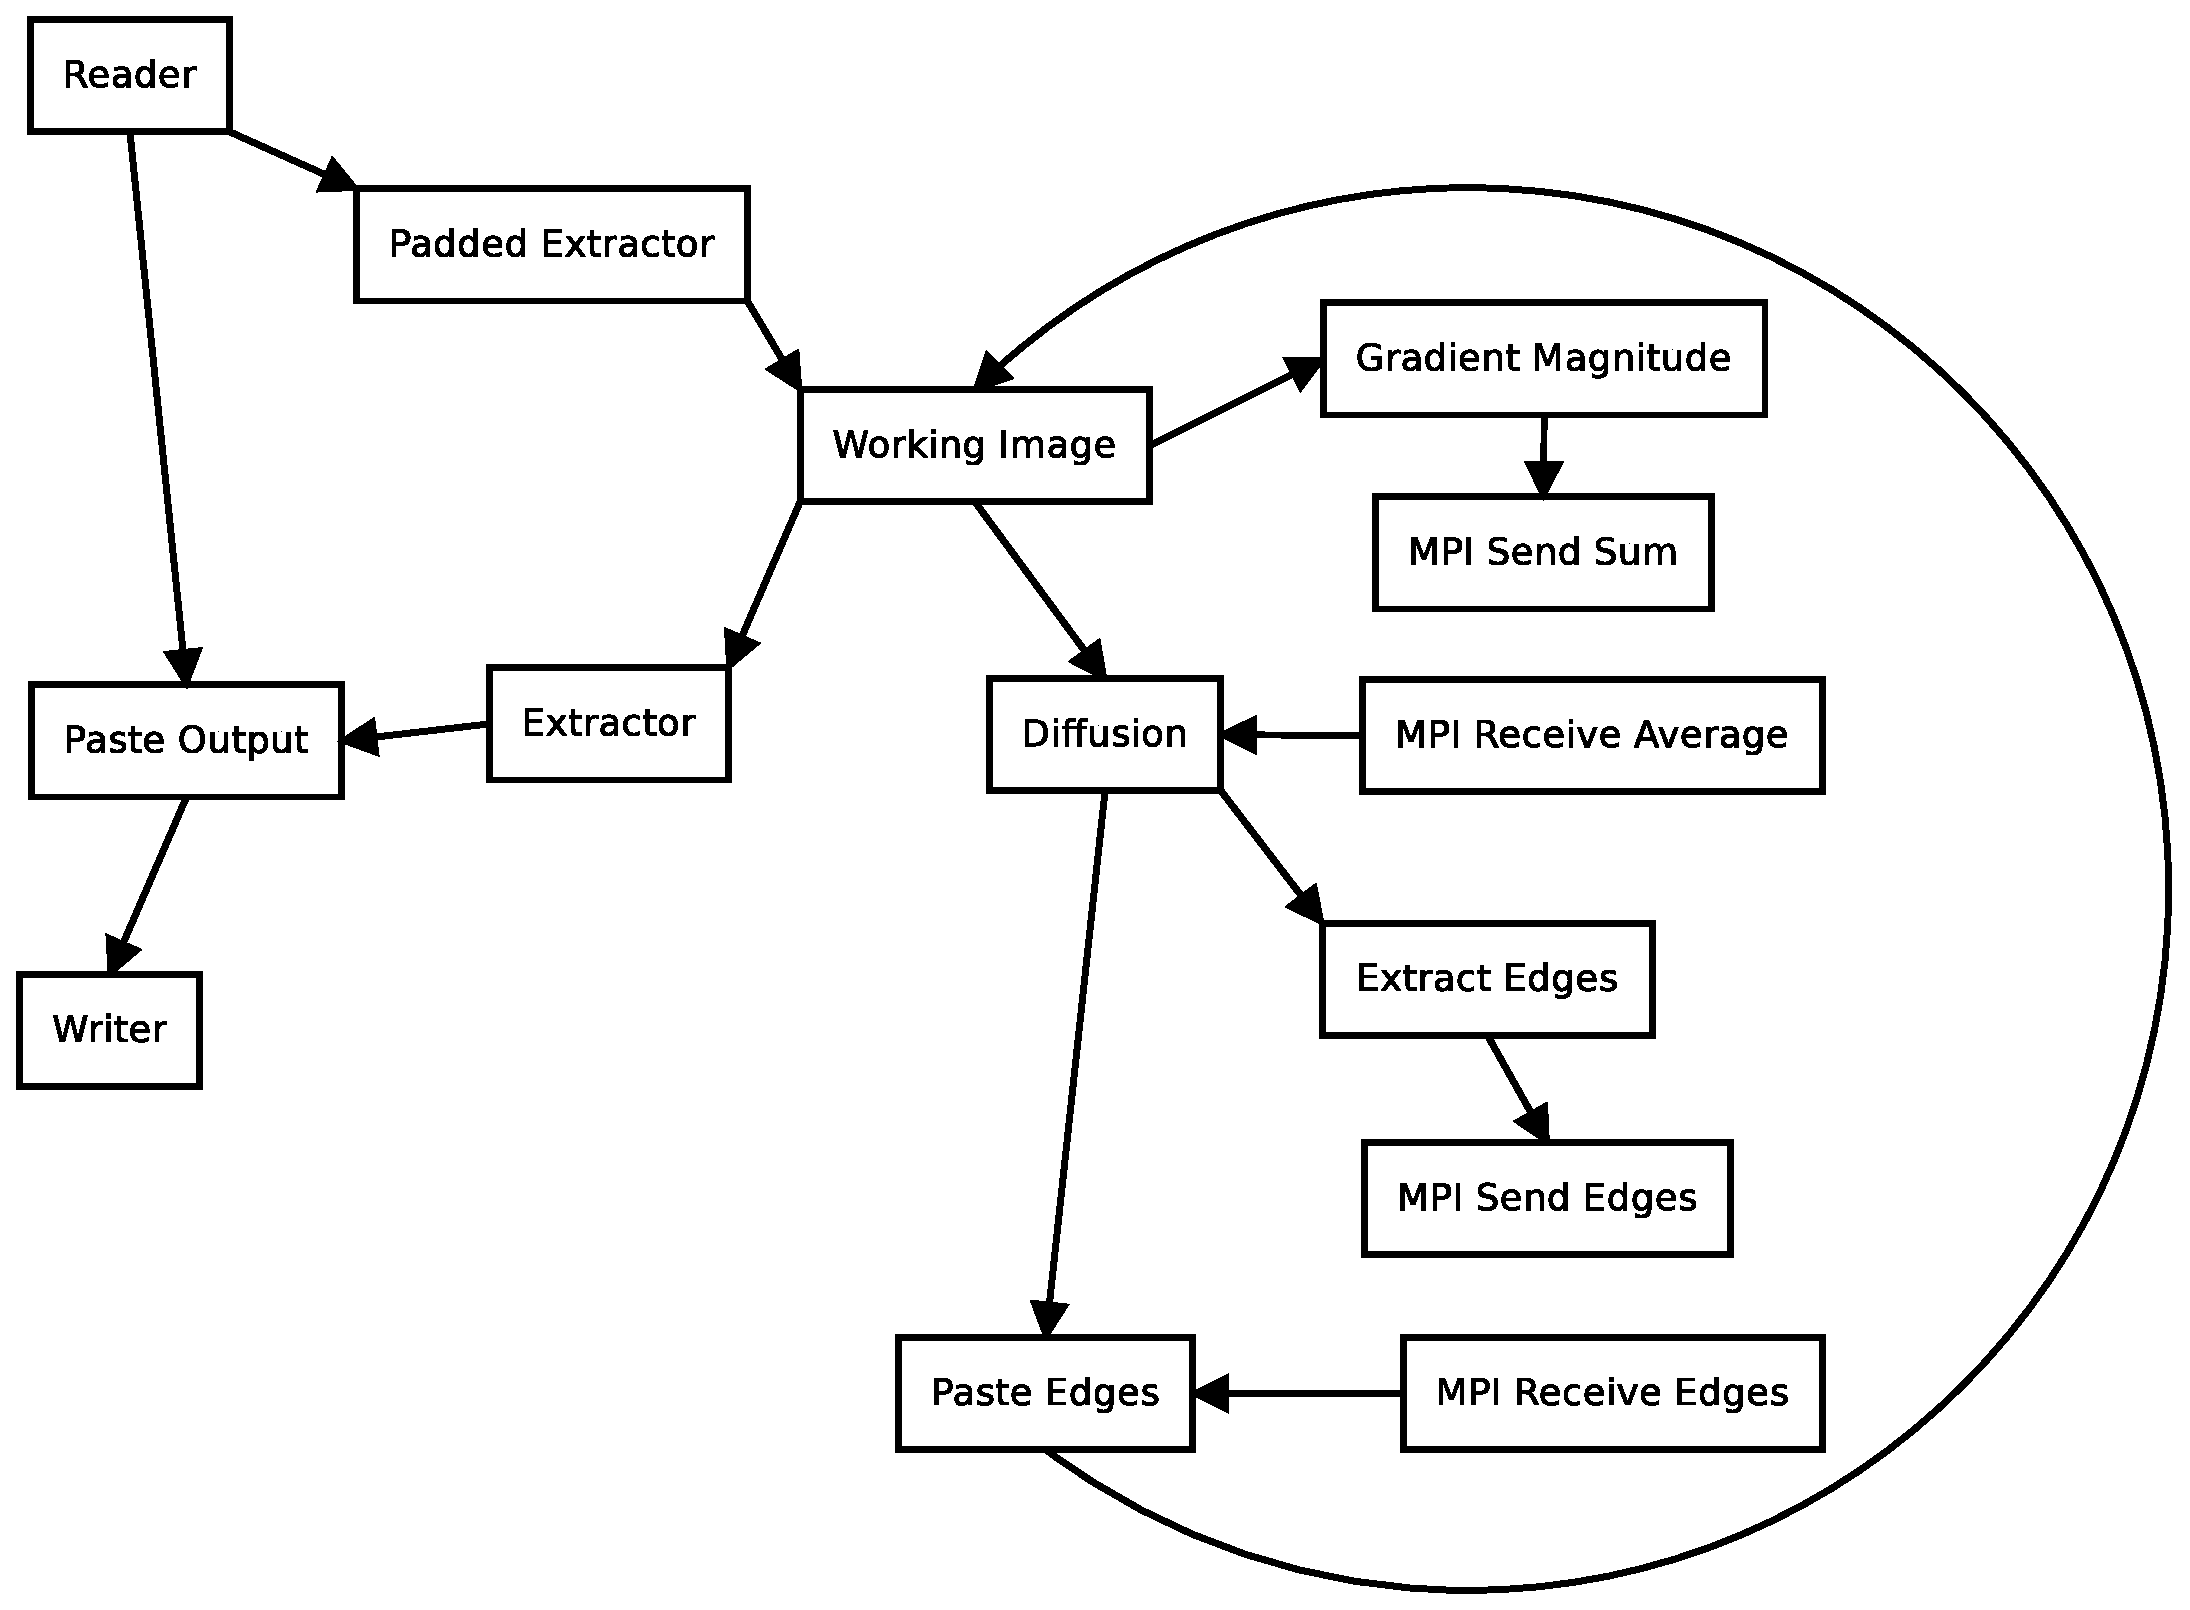
\includegraphics[width=0.8\textwidth]{MPIVectorGradientAnisotropicDiffusionGraph.eps}
\itkcaption[Image Pipeline]{The looping pipeline of 
distributed anisotropic diffusion.}
\label{fig:Image Pipline}
\end{figure}

MPI anisotropic diffusion uses a looping pipeline 
(Figure~\ref{fig:Image Pipline}). Each MPI process is 
responsible for one piece of the total image. Each MPI 
process reads its piece of the input image along with one 
extra pixel of padding in every direction. This padded 
piece is the "Working Image" in 
Figure~\ref{fig:Image Pipline}. Each MPI process 
calculates the gradient magnitude of the padded image and 
sends the sum of all of the pixel values within the region 
for which it is responsible to the first MPI process. Then 
the first MPI process returns the average gradient 
magnitude to every MPI process. The average gradient 
magnitude is used in a single iteration of anisotropic 
diffusion of the working image. Each MPI process sends the 
edges from just within the region for which it is 
responsible of its diffused image to the MPI 
processes responsible for the neighboring pieces and 
receives edges to replace the padding around its piece 
from them (Figure~\ref{fig:Image Overlap}). The updated 
image replaces the "Working Image" and the process is 
repeated. Finally after all iterations are complete, each 
MPI process sends the region of the working image for 
which it is responsible to the first MPI process which 
pastes it into the input image and writes the piece to the 
output file. 

\subsection{Image Overlap}

\begin{figure}
\center
\includegraphics[width=0.8\textwidth]{ImageOverlap.eps}
\itkcaption[Image Overlap]{(1) A one dimensional image is (2) 
split into two regions, one red and one green. (3) The red 
and green regions are padded by one pixel. (4) The red 
region receives the blue pixel from the green region. (5) 
The red region sends the purple pixel to the green region.}
\label{fig:Image Overlap}
\end{figure}

Each pixel in the image piece is influenced by the pixels 
surrounding it during each iteration of anisotropic 
diffusion. To process the pixels on the edges of the piece 
correctly one extra pixel is added to both directions in 
every dimension. After each iteration of anisotropic 
diffusion the values of these pixels must be replaced with 
values from the neighboring pieces. Each MPI process sends 
the values on the edges of its unpadded image piece to 
replace the padding pixel values around the neighboring 
image piece. Each MPI process also receives the pixel 
values from the edge of the neighboring unpadded image 
piece to replace the padding pixel values around its image 
piece (Figure~\ref{fig:Image Overlap}).

\section{Output}

\begin{figure}
\center
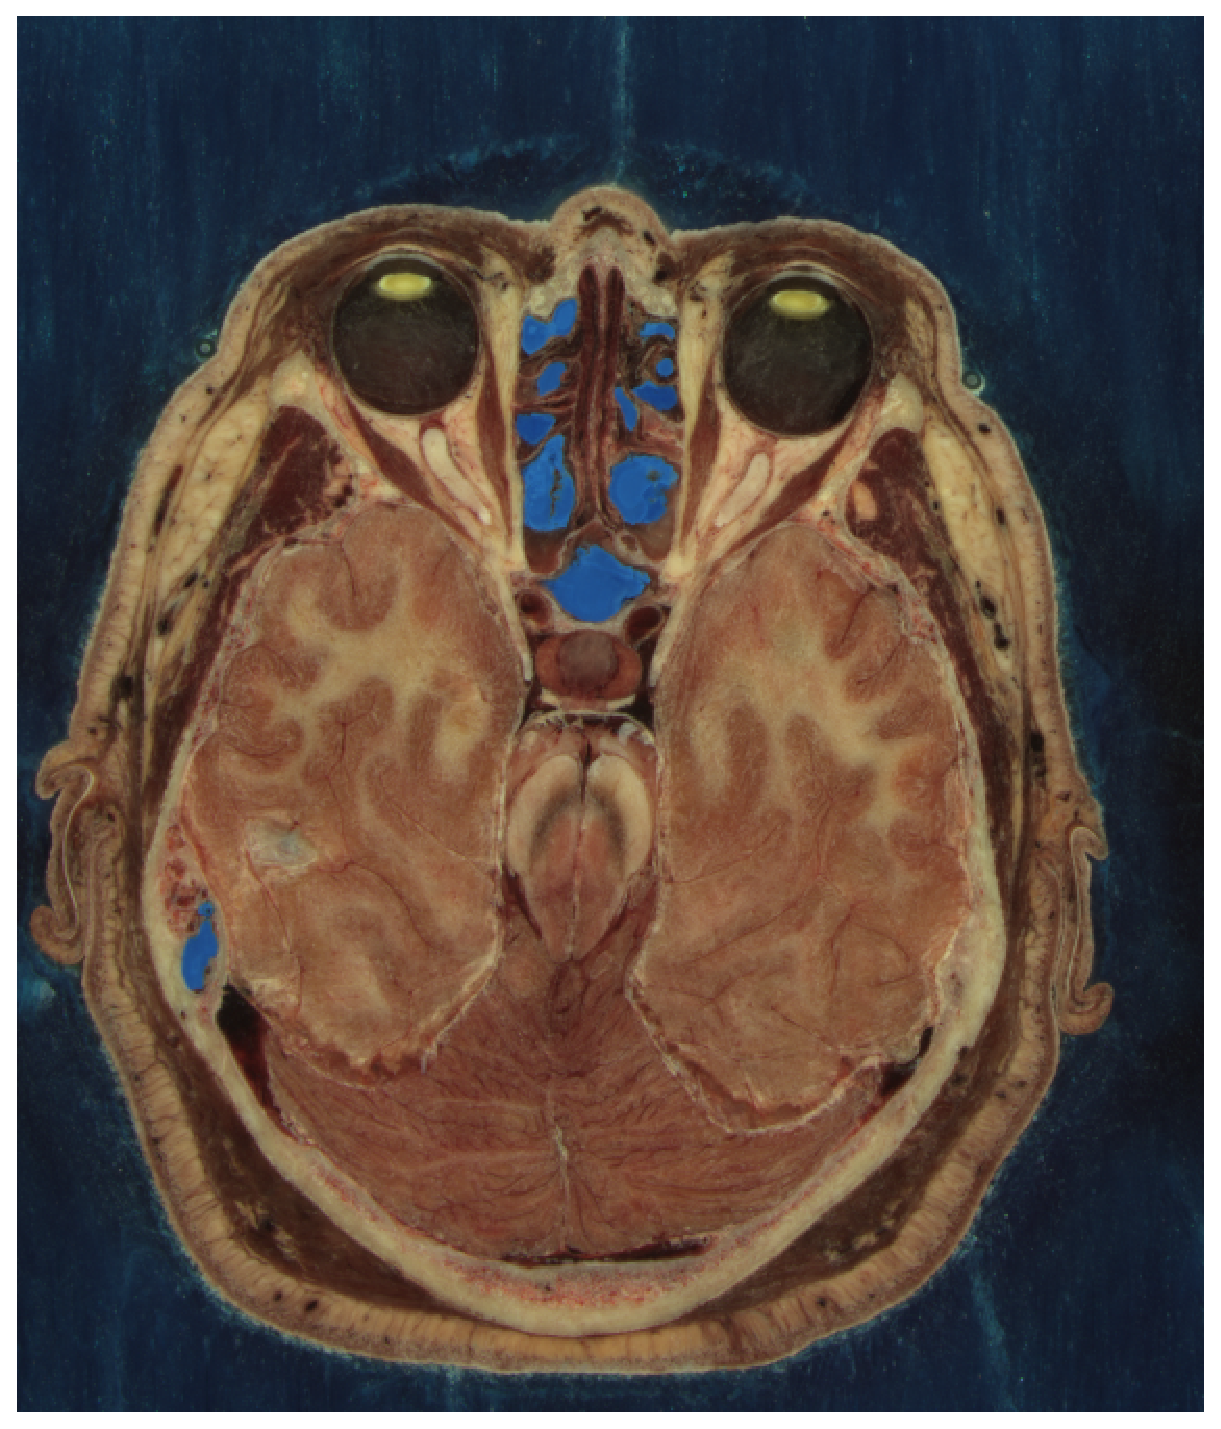
\includegraphics[width=0.8\textwidth]{VisibleWomanHeadFull_Slice.eps}
\itkcaption[Input Image]{A slice of the input image.}
\label{fig:Input Image}
\end{figure}

\begin{figure}
\center
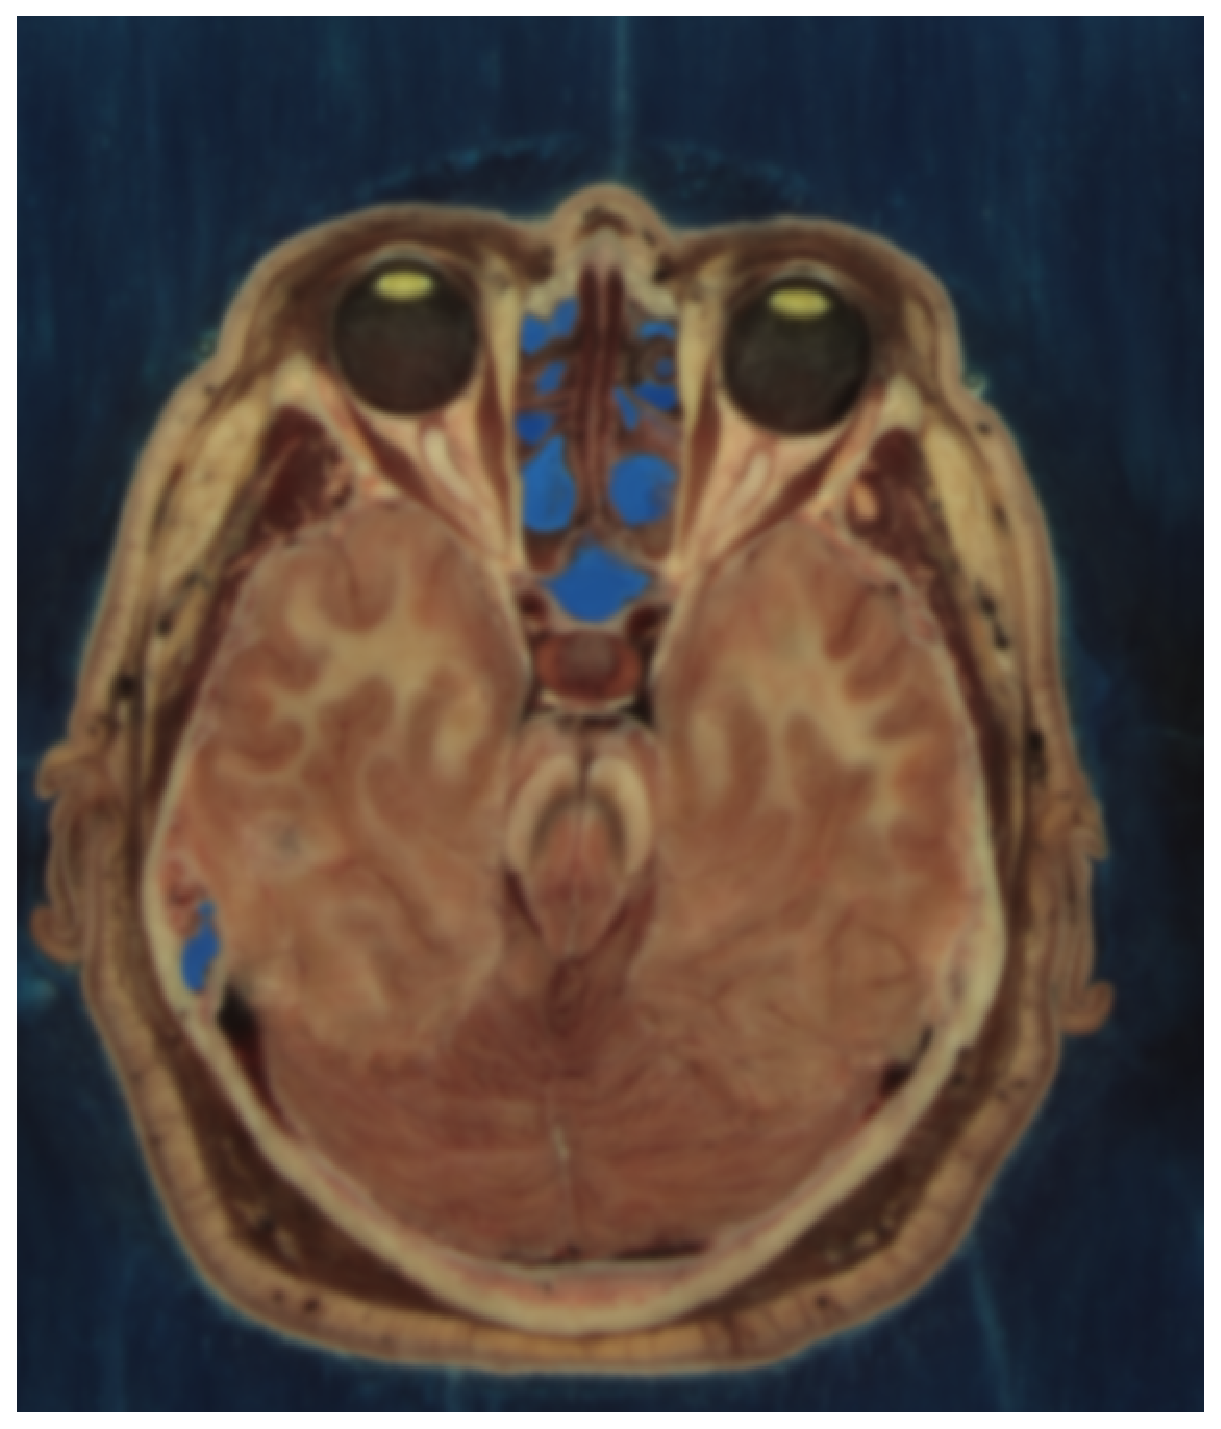
\includegraphics[width=0.8\textwidth]{VisibleWomanHeadFull_Smooth_Slice.eps}
\itkcaption[Output Image]{A slice of the output image.}
\label{fig:Output Image}
\end{figure}

Figure~\ref{fig:Input Image} shows one slice of an input 
image which was processed using the ITK vector gradient 
magnitude anisotropic diffusion filter inside of the 
distributed anisotropic diffusion program. The program 
took 47 minutes to process the image. The computer was an 
eight node cluster. Each node had two Intel Xeon X5550 
2.67GHz processors with four cores each and 12 GB of RAM. 
The nodes were connected with gigabit Ethernet. One MPI 
process was started on each node with ITK's 
multi-threading using all processor cores. The parameters 
were conductance parameter~=~0.2, iterations~=~100, and 
time step~=~0.015. Figure~\ref{fig:Output Image} shows a 
slice of the output image.

\section{Scaling}

\begin{figure}
\center
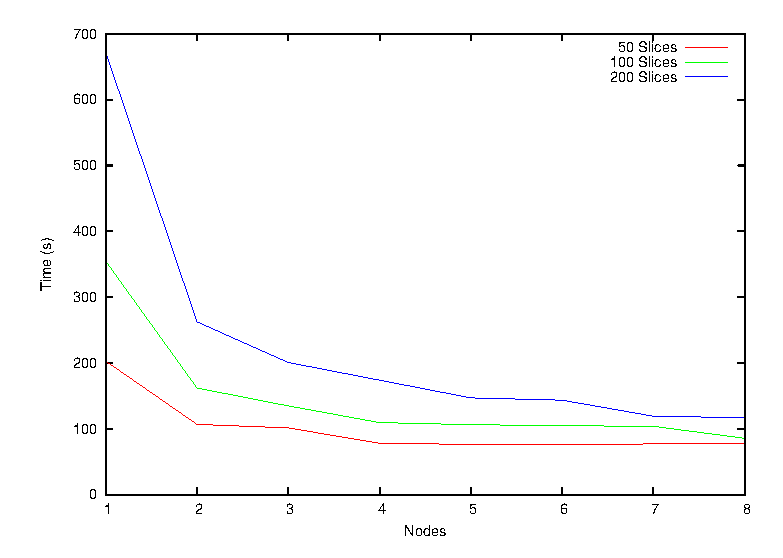
\includegraphics[width=0.8\textwidth]{time.eps}
\itkcaption[Processing Times]{Processing times with three 
different data sizes for 10 iterations of standard (1 node) and distributed 
($\geq$ 2 nodes) vector gradient magnitude anisotropic diffusion}
\label{fig:Processing Times}
\end{figure}

When run on 50, 100, and 200 slice slabs of the Visible 
Woman Head data set with conductance parameter~=~0.2, 
iterations~=~10, and time step~=~0.015 standard vector 
gradient magnitude anisotropic diffusion always took 
more time than the distributed version 
(Figure~\ref{fig:Processing Times}). Adding more than 4 
nodes did not greatly decrease processing time until the 
200 slice data set.

\section{Software Used}

This program was built using :

% The {itemize} environment uses a bullet for each \item.  If you want the 
% \item's numbered, use the {enumerate} environment instead.
\begin{itemize}
  \item  Insight Toolkit ( GIT )
  \item  CMake ( GIT )
  \item  MPI ( openmpi-1.4.3 )
\end{itemize}

\section{Acknowledgements}

This work was done in Scott L. Hooper's lab at Ohio University 
hooper@ohio.edu. 

The Visible Woman Head data set used in 
Figs.~\ref{fig:Input Image},~\ref{fig:Output Image}, and the 
piece used in the tests that accompany this paper was 
downloaded from 
\url{http://public.kitware.com/pub/itk/Data/VisibleWomanHead/RawRGB/}

This work was funded by NSF Award \# IOS-0958926 and NIH 
Award \# ARRA-RC1DA028494.



% The preceding sections will have been written in a gentler,
% introductory style.  You may also wish to include a reference
% section, documenting all the functions/exceptions/constants.
% Often, these will be placed in separate files and input like this:



%%%%%%%%%%%%%%%%%%%%%%%%%%%%%%%%%%%%%%%%%
%
%  Insert the bibliography using BibTeX
%
%%%%%%%%%%%%%%%%%%%%%%%%%%%%%%%%%%%%%%%%%


\end{document}

